
%version 2: \usepackage{hyperref}


%%%%%%%%%%%%%%%%%%%%%%%%%%%%%%%%%%%%%%%%%%%%%%%%%%%%%%%%%%%%%%%%%%%%%%%%
%Para las ecuaciones siempre es Ec.(n).
%Para las figuras siempre es Fig.n, incluso en el caption de la figura. Tambien las Tablas
%Para las referencias es [n]
%%%%%%%%%%%%%%%%%%%%%%%%%%%%%%%%%%%%%%%%%%%%%%%%%%%%%%%%%%%%%%%%%%%%%%%%

\documentclass[
reprint,
%notitlepage,
%superscriptaddress,
%groupedaddress,
%unsortedaddress,
%runinaddress,
%frontmatterverbose, 
%preprint,
%showpacs,preprintnumbers,
%nofootinbib,
%nobibnotes,
%bibnotes,
%11 pt,
amsmath,
amssymb,
%aps,
%pra,
prb,
%rmp,
%tightenlines %esto hizo el milagro de sacar los espacios en blancos estocásticos (?)
%prstab,
%prstper,
%floatfix,\textbf{}
]{revtex4-1} %Instalar primero para usarlo. Paquete malo.

%\documentclass[onecolumn, aps, amsmath,amssymb ]{article}
\usepackage{lipsum}  
\usepackage{graphicx}% Include figure files
\usepackage{subfig}
\usepackage{braket}
\usepackage{comment} %comment large chunks of text
\usepackage{dcolumn}% Align table columns on decimal point
\usepackage{bm}% bold math
%\usepackage{hyperref}% add hypertext capabilities
\usepackage[mathlines]{lineno}% Enable numbering of text and display math
%\linenumbers\relax % Commence numbering lines
\usepackage{mathtools} %% Para el supraíndice

\usepackage[nice]{nicefrac}

%%%%%%%El Señor Español%%%%%%%%%%%%%%%%%%%%%%%%%%%
\usepackage[utf8]{inputenc} %acento
\usepackage[
spanish, %El lenguaje.
es-tabla, %La tabla y no cuadro.
activeacute, %El acento.
es-nodecimaldot %Punto y no coma con separador de números
]{babel}
\usepackage{microtype} %para hacerlo más bonito :33 como vos (?) 
%%%%%%%%%%%%%%%%%%%%%%%%%%%%%%%%%%%%%%%%%%%%%%%%%%%
%%%%%%%%% Para que las imágenes se queden dónde las quiero (?
\usepackage{float}
%%%%%%%%%%
\usepackage{enumitem}
\usepackage{hyperref} % Para usar \url

%%%%%%%%Cambia a Fig de Figure%%%%%%%%%%
\makeatletter
\renewcommand{\fnum@figure}{Fig. \thefigure} 
\makeatother
%%%%%%%%%%%%%%%%%%%%%%%%%%%%%%%%%%%%%%%%
\raggedbottom
 
\begin{document}

\title{Práctica 7: Redes Neuronales Recurrentes }
\author{Evelyn G. Coronel}

\affiliation{Redes Neuronales y Aprendizaje Profundo para Visión Artificial\\ Instituto Balseiro\\}

\date[]{\lowercase{\today}} 

\maketitle

\section*{Ejercicio 1}
\subsection*{Item 1}

Los datos representan la cantidad de pasajeros de aviones por mes desde Enero del 1949 hasta el mes de Diciembre del 1960. Estos datos tienen una oscilación anual y crecimiento en función del tiempo como se ven en la Fig.\,\ref{fig:datos}.

\begin{figure}[H]
	\begin{small}
		\begin{center}
			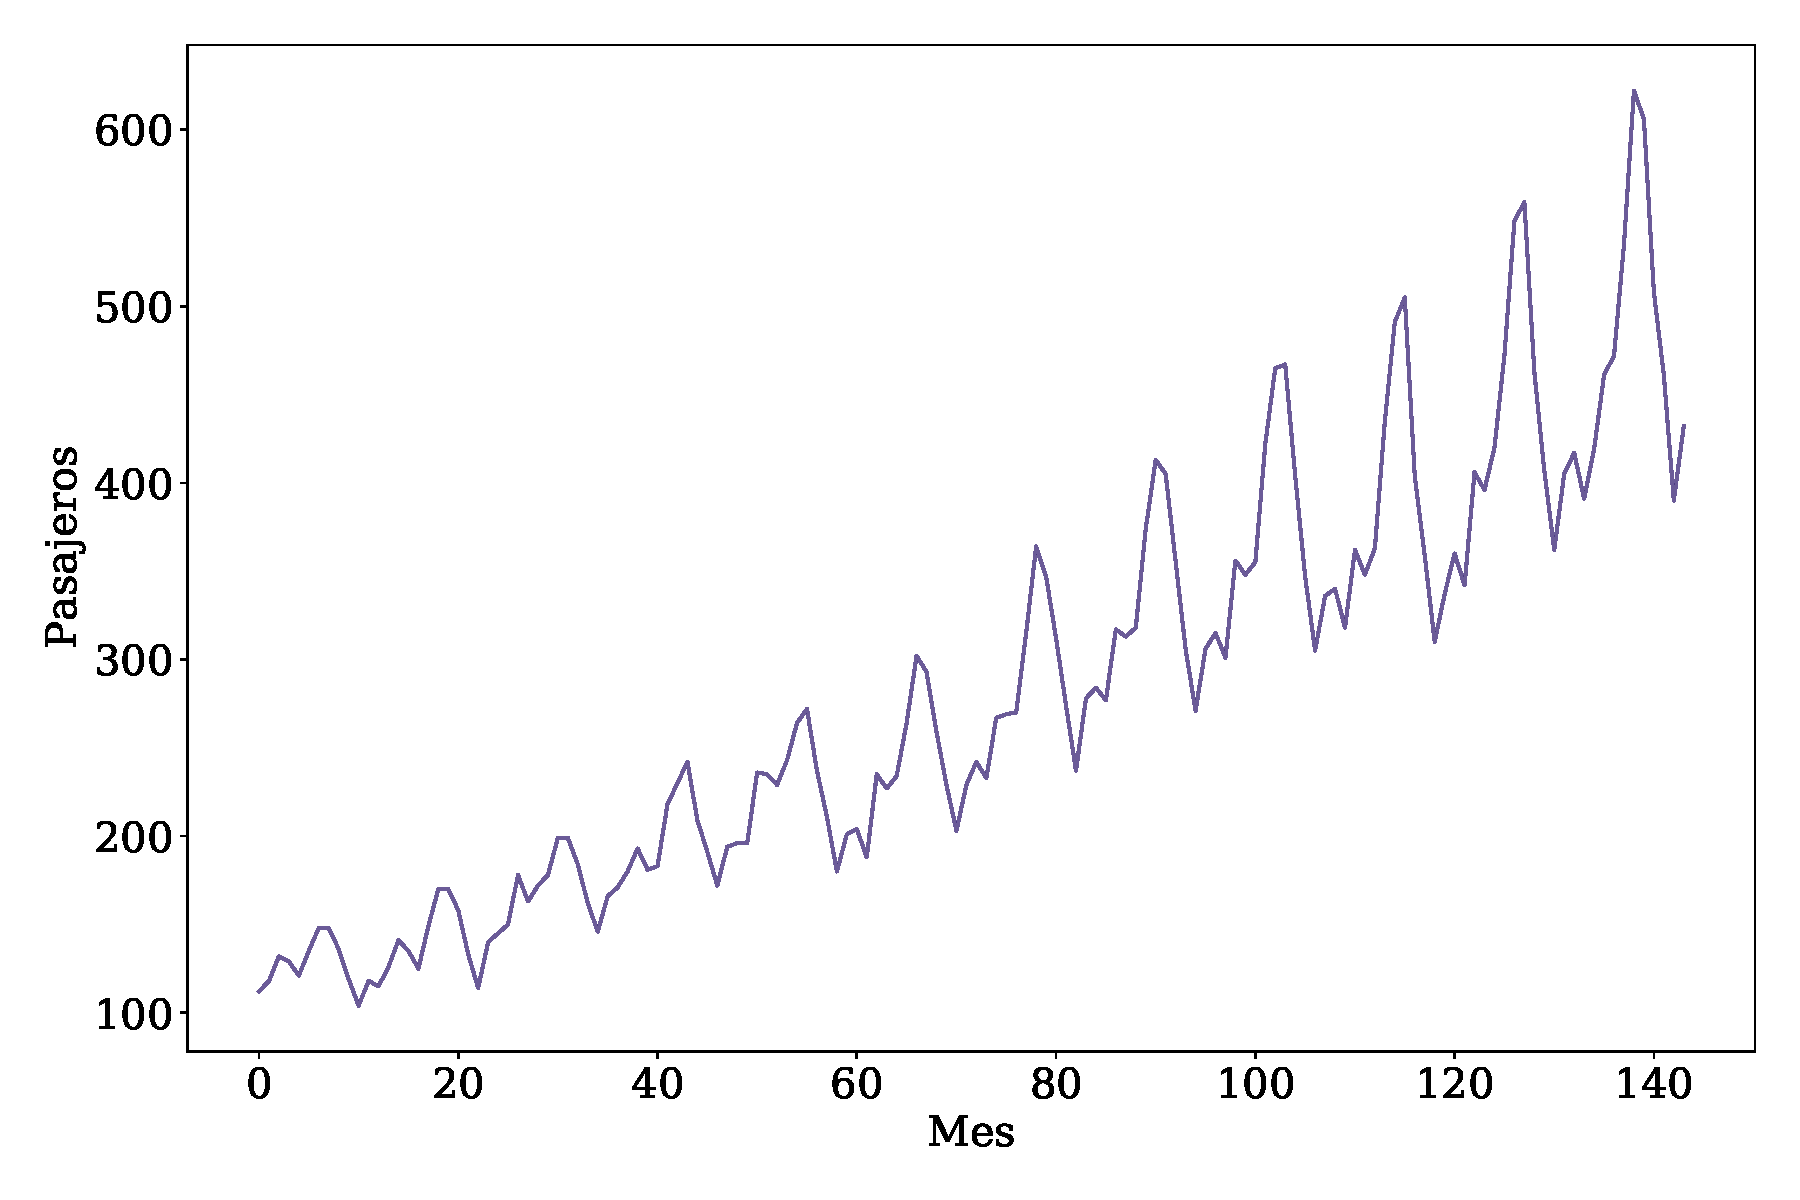
\includegraphics[width=0.45\textwidth]{datos.pdf}
		\end{center}
		\caption{Cantidad de pasajeros en función de los meses a partir de Enero del 1949}
		\label{fig:datos}
	\end{small}
\end{figure}


\subsection*{Item 2}

Para utilizar estos datos para predecir la cantidad de pasajeros en función del tiempo, en el preprocesado se normalizaron los datos de tal forma que varíen entre $0-1$. 

Tomando el set de datos como $x(t)$ donde x representa la cantidad de pasajeros y $t$ representa el mes, se organiza los datos según el desfase $l$ que representa la cantidad de meses y se formatean según el siguiente algoritmo:

\begin{itemize}
\item Si  $l=1$:
	\begin{align*}
		X = x(t) \qquad Y = x(t+1)
	\end{align*}
\item 	 Si $l=2$:
	Por ejemplo si queremos obtener $Y$ para el primer  elemento $x(0)$, obtenemos los siguientes vectores:
	\begin{align*}
		X = \big ( x(0), x(1) \big ) \qquad Y = x(2)
	\end{align*}
	Generalizando para cualquier $t$:
	\begin{align*}
		X = \big ( x(t), x(t+1) \big ) \qquad Y = x(t+2)
	\end{align*}
\item 	 Para $l$ arbitrario:
	Generalizando para cualquier $\tilde{t}$:
	\begin{align*}
		X = \big ( x(t), x(t+1),\cdots, x(t+l-1) \big ) \qquad Y = x(t+l)
	\end{align*}

\end{itemize}

Los datos se formatean de esta forma para hacer que la red aprenda a predecir la cantidad de pasajeros el mes $A$, utilizando la información considerando los $l$ meses anteriores

\subsection*{Items 3, 4 y 5}

Se agrega el ruido gaussiano para probar si la red es capaz de aprender el patrón de la cantidad de pasajeros a pesar del ruido. 

Para entrenar la red recurrente, se separaron los datos de entrenamiento y test en $70\%$ y $30\%$ respectivamente. 

Dado que nuestros conjunto de datos solo contiene la cantidad de pasajeros, por que al redimensionar los datos para la entrada del LSTM, se considera que cantidad de atributos  (\emph{features}) es 1 y el rango de tiempo utilizado para hacer el entrenamiento de $l$ meses.

\subsection*{Item 6 y 7}

Las arquitectura de la red utilizada para predecir la cantidad de pasajeros son:  una capa LSTM con 4 entradas y una salida de 1, y otra red con una capa densa de 4 neuronas con una salida de 1.

Se utilizó el optimizador Adam con una tasa de aprendizaje de $2\times10^{-3}$ y MSE como función de pérdida para ambas redes, las mismas fueron entrenadas durante 100 épocas.

\subsection*{Item 8 y 10}

Entrenando la red con $l=1$ se obtiene las predicciones (V) usando la capa LSTM mostrado en la Fig.\,\ref{fig:l-1-LSTM} junto a los datos de entrenamiento (E), en caso de la red con la capa densa estas curvas se muestran en la Fig.\,\ref{fig:l-1-Densa}. La pérdidas normalizadas de estas redes se muestran en las Figs.\, respectivamente, los datos de entrenamiento llegan a un valor de $MSE=0.0023$ mientras que la test $MSE=0.012$ con la capa de entrada del tipo LSTM, cuando pasamos a la otra red el valor de $MSE$ para el  entrenamiento es $0.0024$ y para la test $0.010$. En este trabajo para $l=1$, la red con capas densas da una mejor predicción que la red LSTM.

\begin{figure}[H]
	\begin{small}
		\begin{center}
			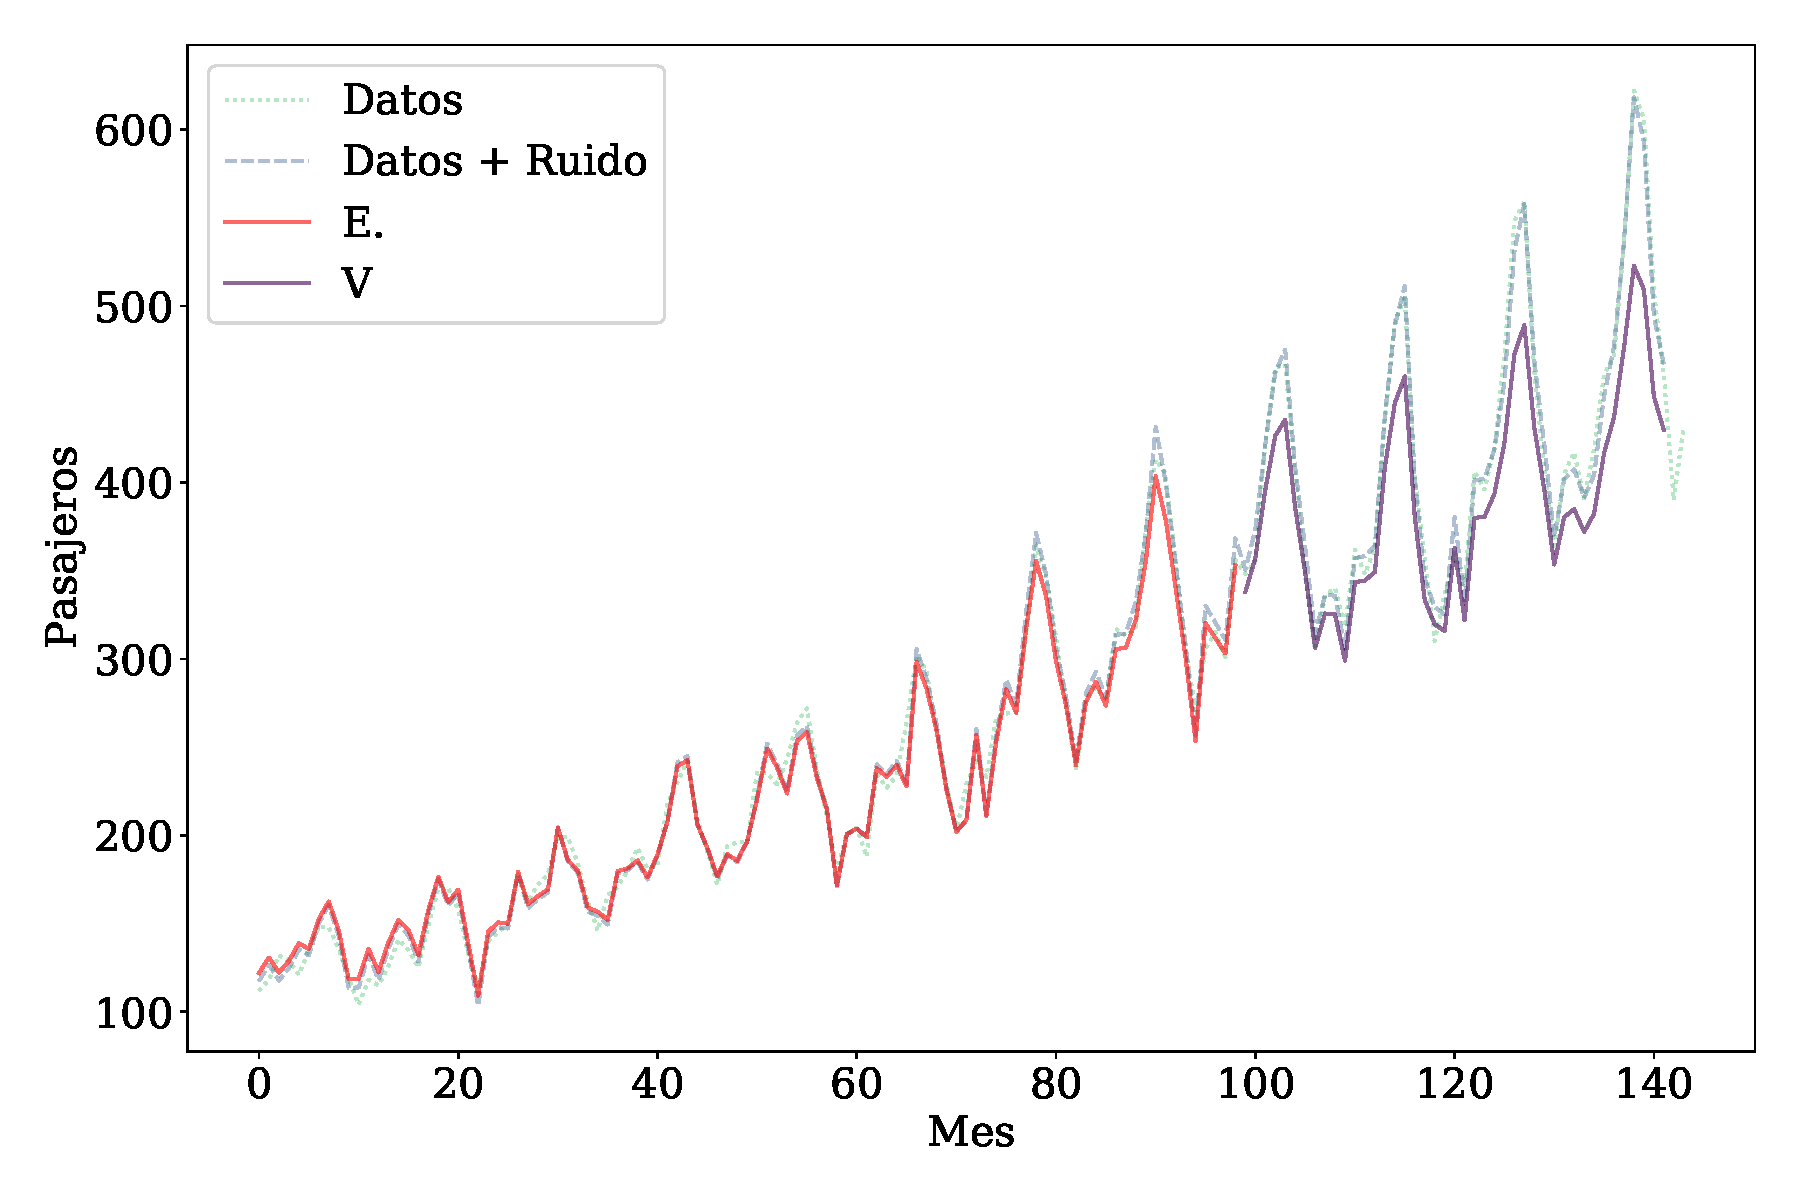
\includegraphics[width=0.5\textwidth]{prediccion_l-1.pdf}
		\end{center}
		\caption{Predicción de la cantidad de pasajeros usando un desfase de 1 mes para el entrenamiento usando una capa LSTM}
		\label{fig:l-1-LSTM}
	\end{small}
\end{figure}


\begin{figure}[H]
	\begin{small}
		\begin{center}
			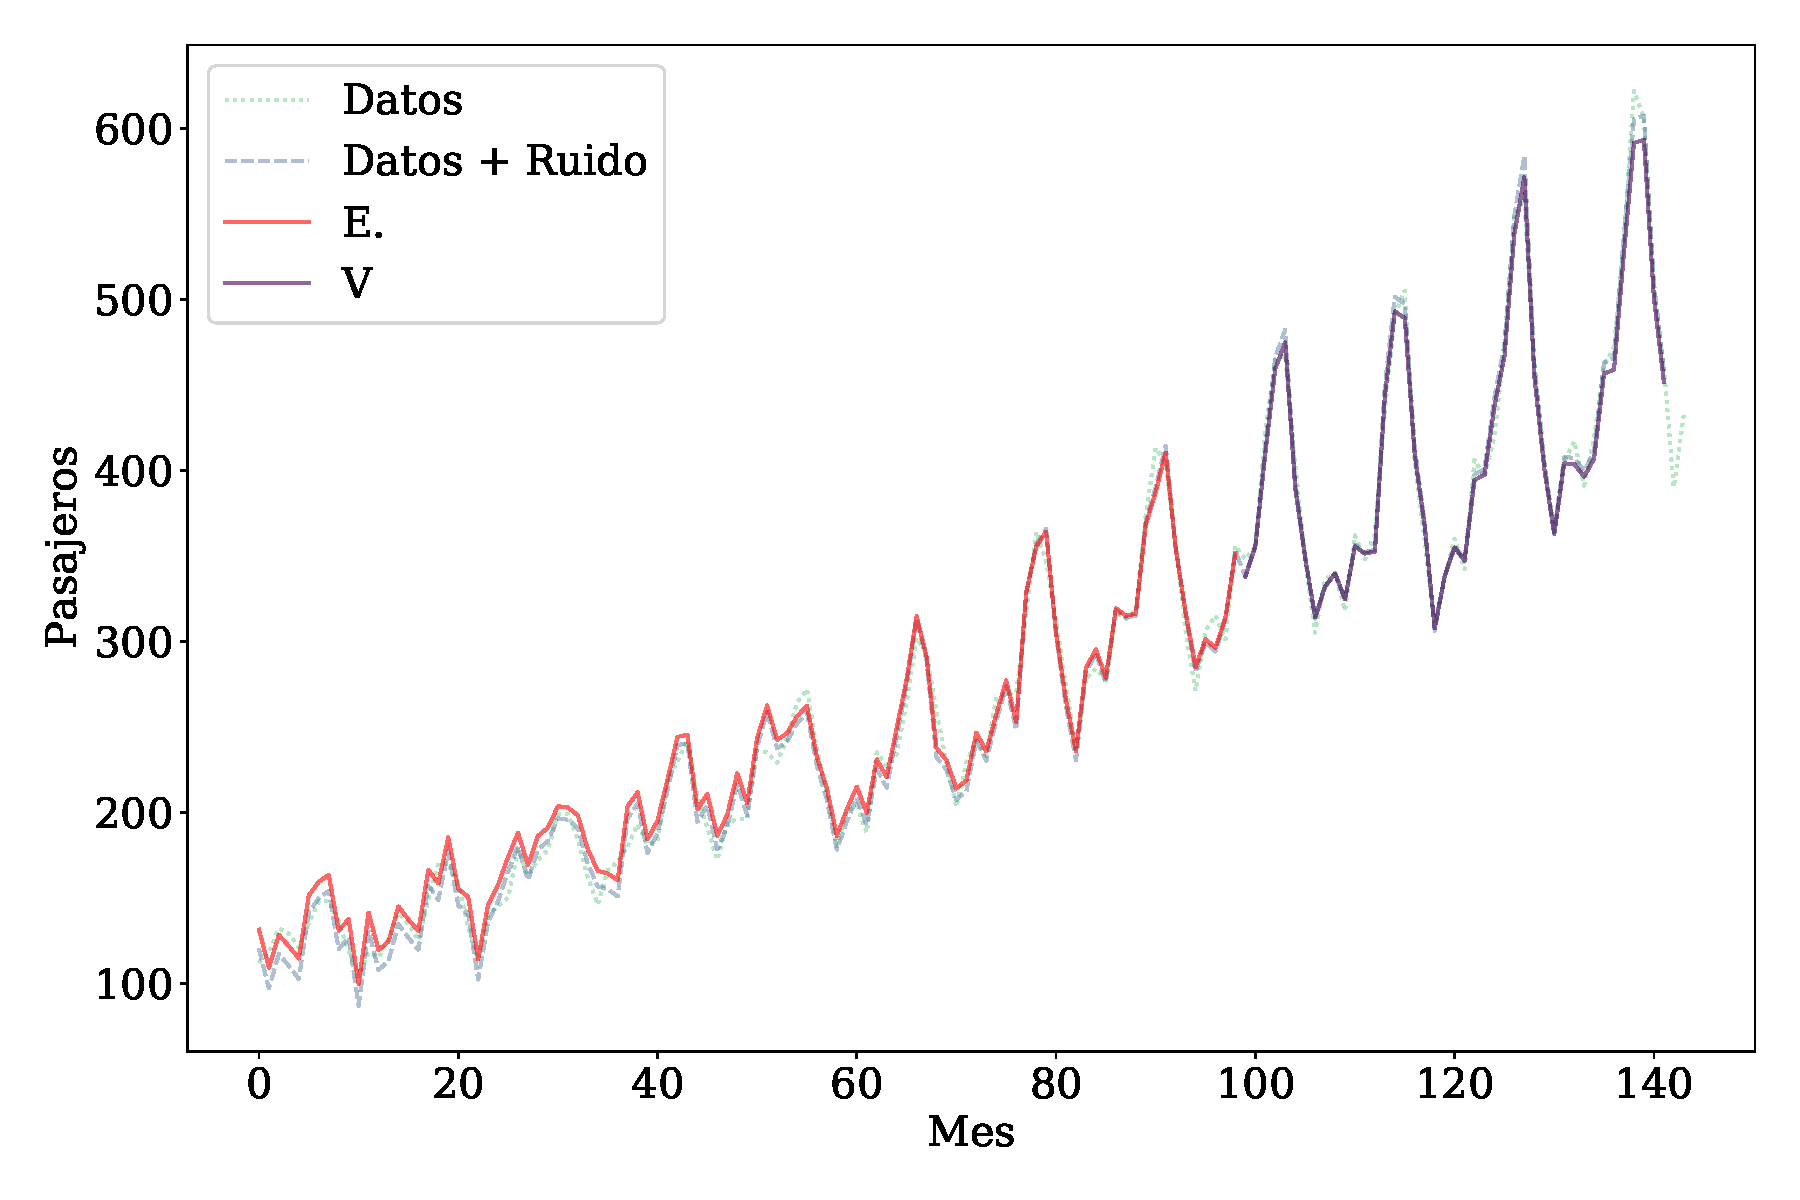
\includegraphics[width=0.5\textwidth]{prediccion_l-1_dense.pdf}
		\end{center}
		\caption{Predicción de la cantidad de pasajeros usando un desfase de 1 mes para el entrenamiento usando una capa densa}
		\label{fig:l-1-Densa}
	\end{small}
\end{figure}

Considerando que las variaciones de la cantidad de pasajeros tiene una modulación de 12 meses, este trabajo utilizó $l=13$ para ver como funciona con red prediciendo las cantidad de pasajeros con los 13 meses anteriores. La predicción se muestra en la Fig.\ref{fig:l-13-LSTM} , donde se muestra que la red predice  mejor  los picos el caso de $l=1$.


\begin{figure}[H]
	\begin{small}
		\begin{center}
			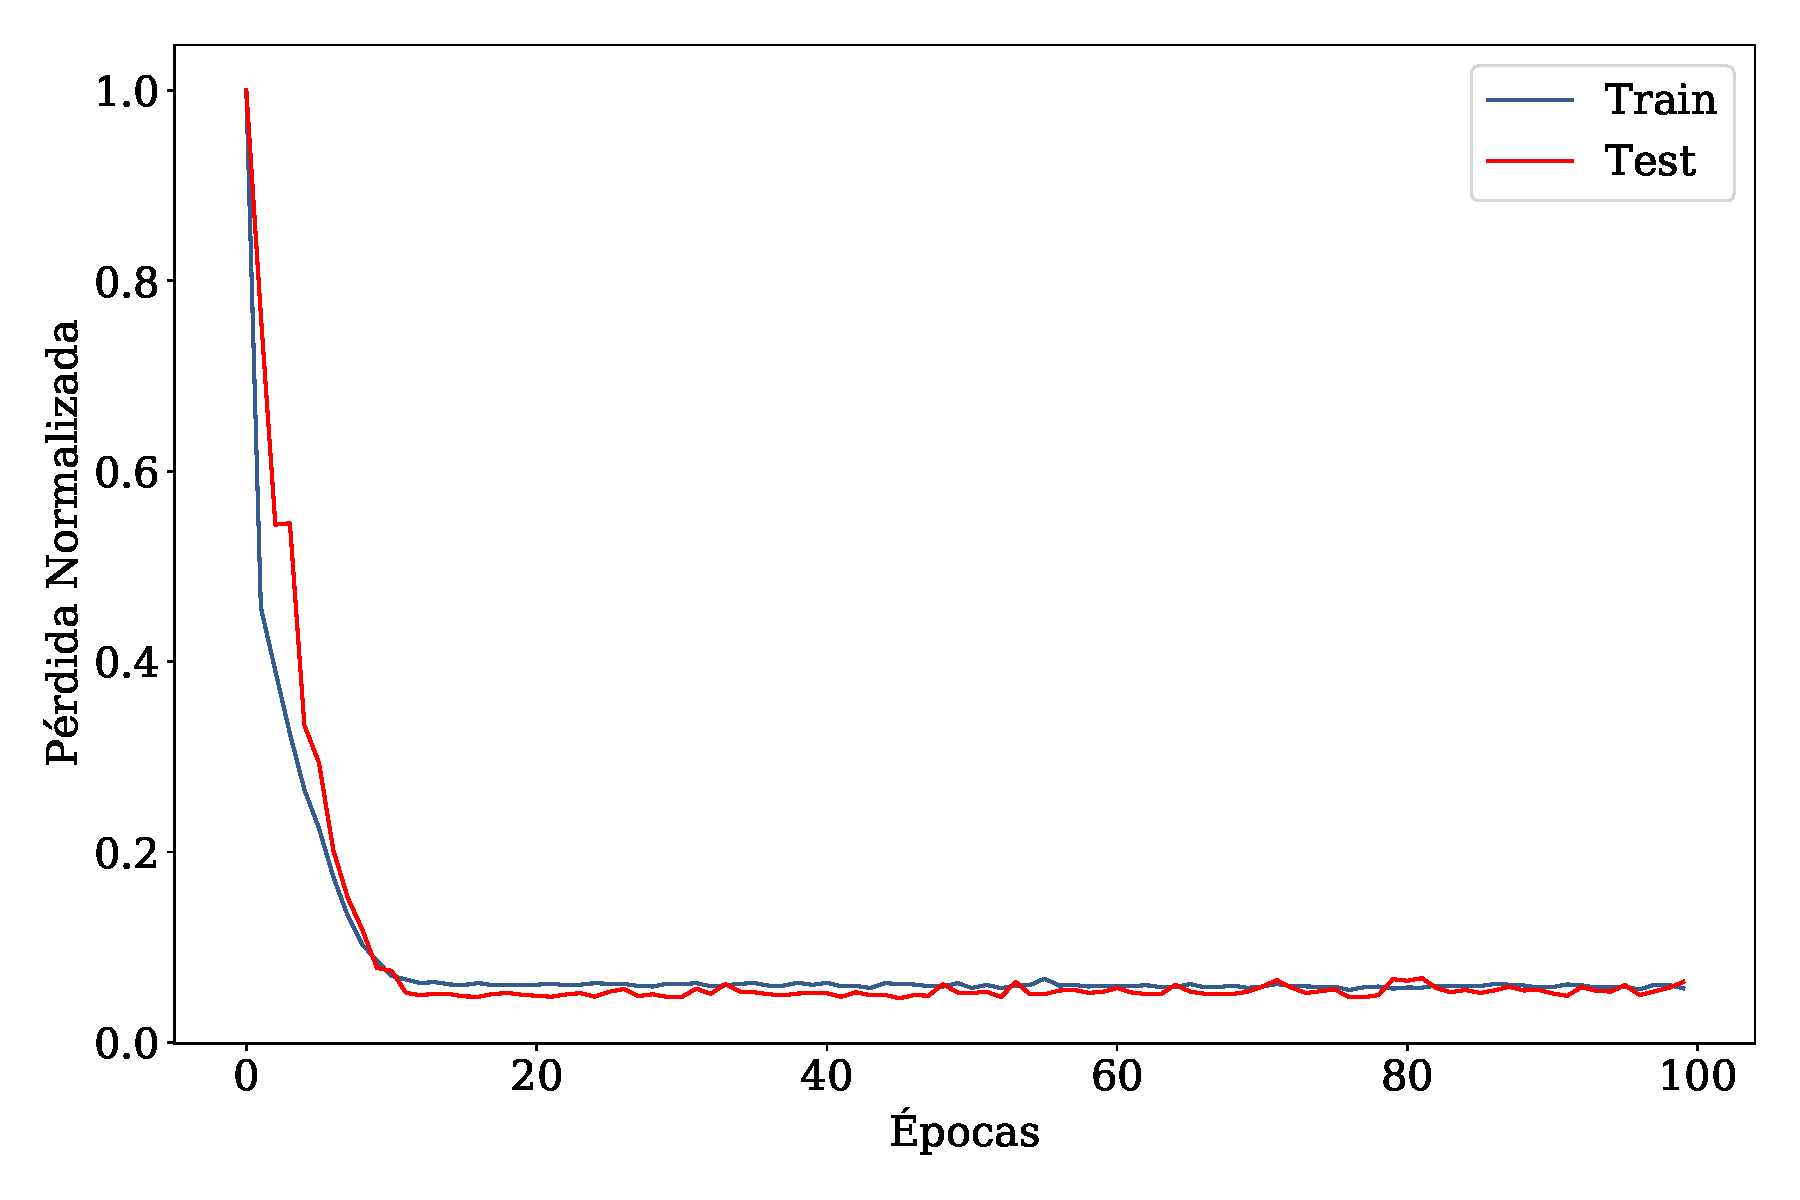
\includegraphics[width=0.5\textwidth]{prediccion_l-1_loss.pdf}
		\end{center}
		\caption{Pérdida en función de las épocas usando un desfase de 1 mes para el entrenamiento usando una capa LSTM}
		\label{fig:l-1-LSTM}
	\end{small}
\end{figure}


\begin{figure}[H]
	\begin{small}
		\begin{center}
			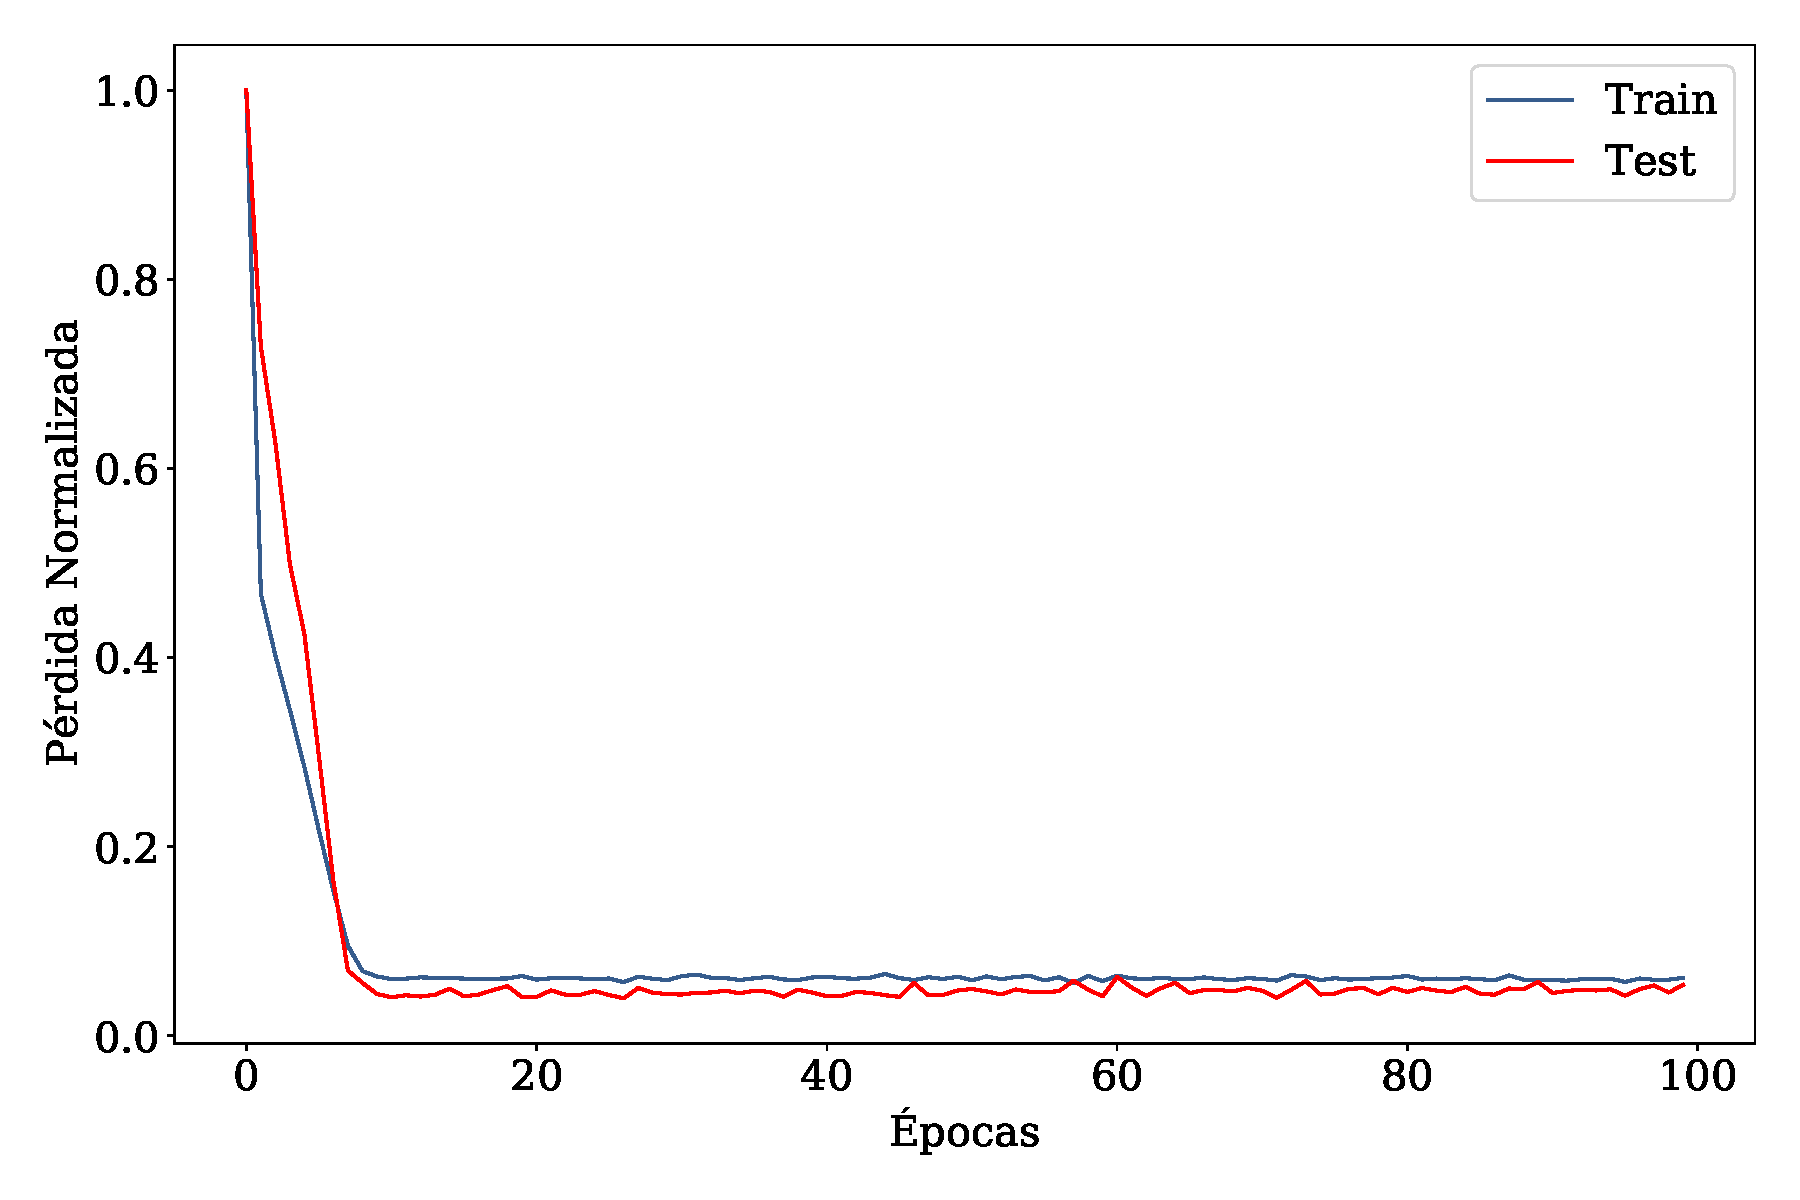
\includegraphics[width=0.5\textwidth]{prediccion_l-1_dense_loss.pdf}
		\end{center}
		\caption{Pérdida en función de las épocas usando un desfase de 1 mes para el entrenamiento usando una capa densa}
		\label{fig:l-1-Densa}
	\end{small}
\end{figure}


\subsection*{Item 9}

Por lo observado en los items anteriores, la predicción de la red depende de cuanto fue el desfase de tiempo dado para el entrenamiento. En la Fig.\,\ref{fig:barrido_en_l} se muestra el valor de MSE del test en función del parámetros $l$. Se observa un mínimo del valor del MSE en los desfases corridos en un año, esto se debe a la periodicidad del conjunto de datos.

\begin{figure}
	\begin{small}
		\begin{center}
			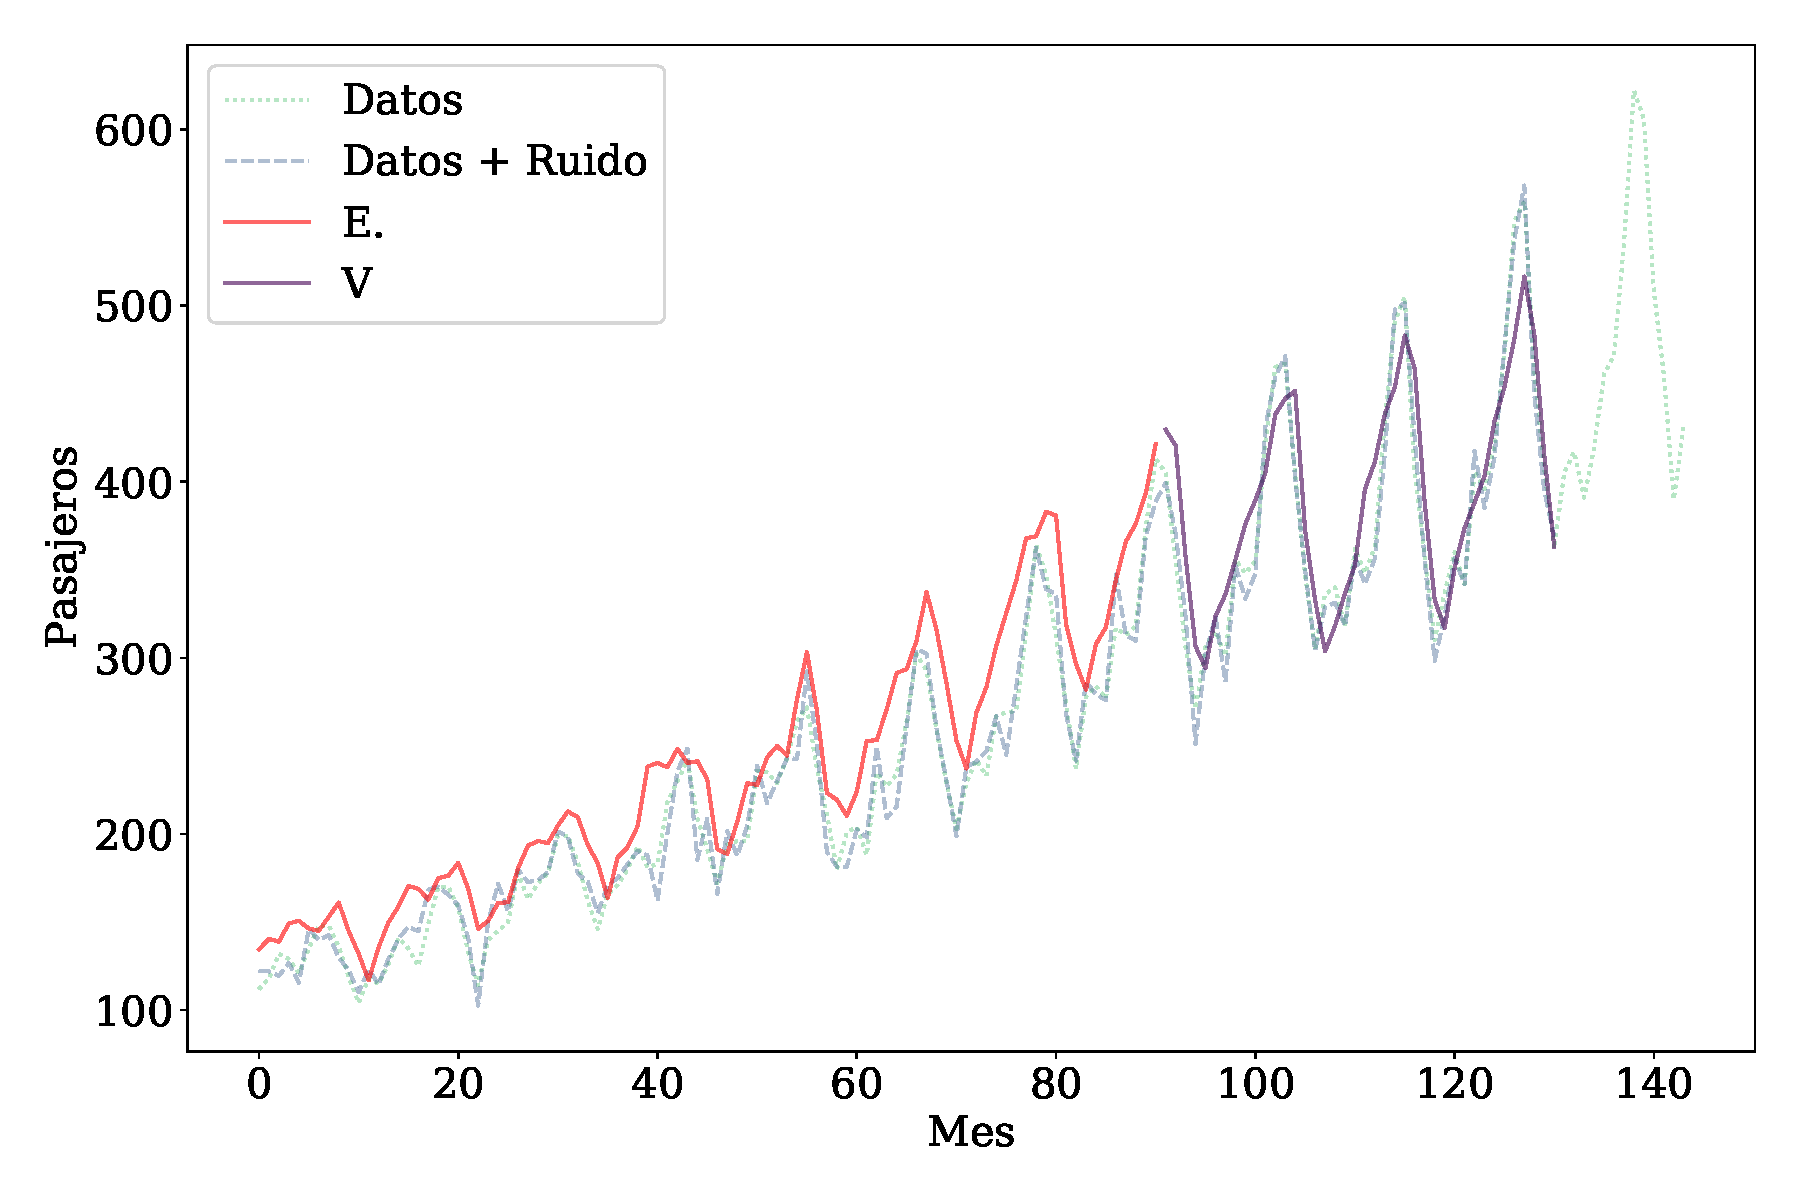
\includegraphics[width=0.5\textwidth]{prediccion_l-12.pdf}
		\end{center}
		\caption{Predicción de la cantidad de pasajeros usando un desfase de 13 meses para el entrenamiento usando una capa LSTM}
		\label{fig:l-13-LSTM}
	\end{small}
\end{figure}
\vfill \null 
\begin{figure}[H]
	\begin{small}
		\begin{center}
			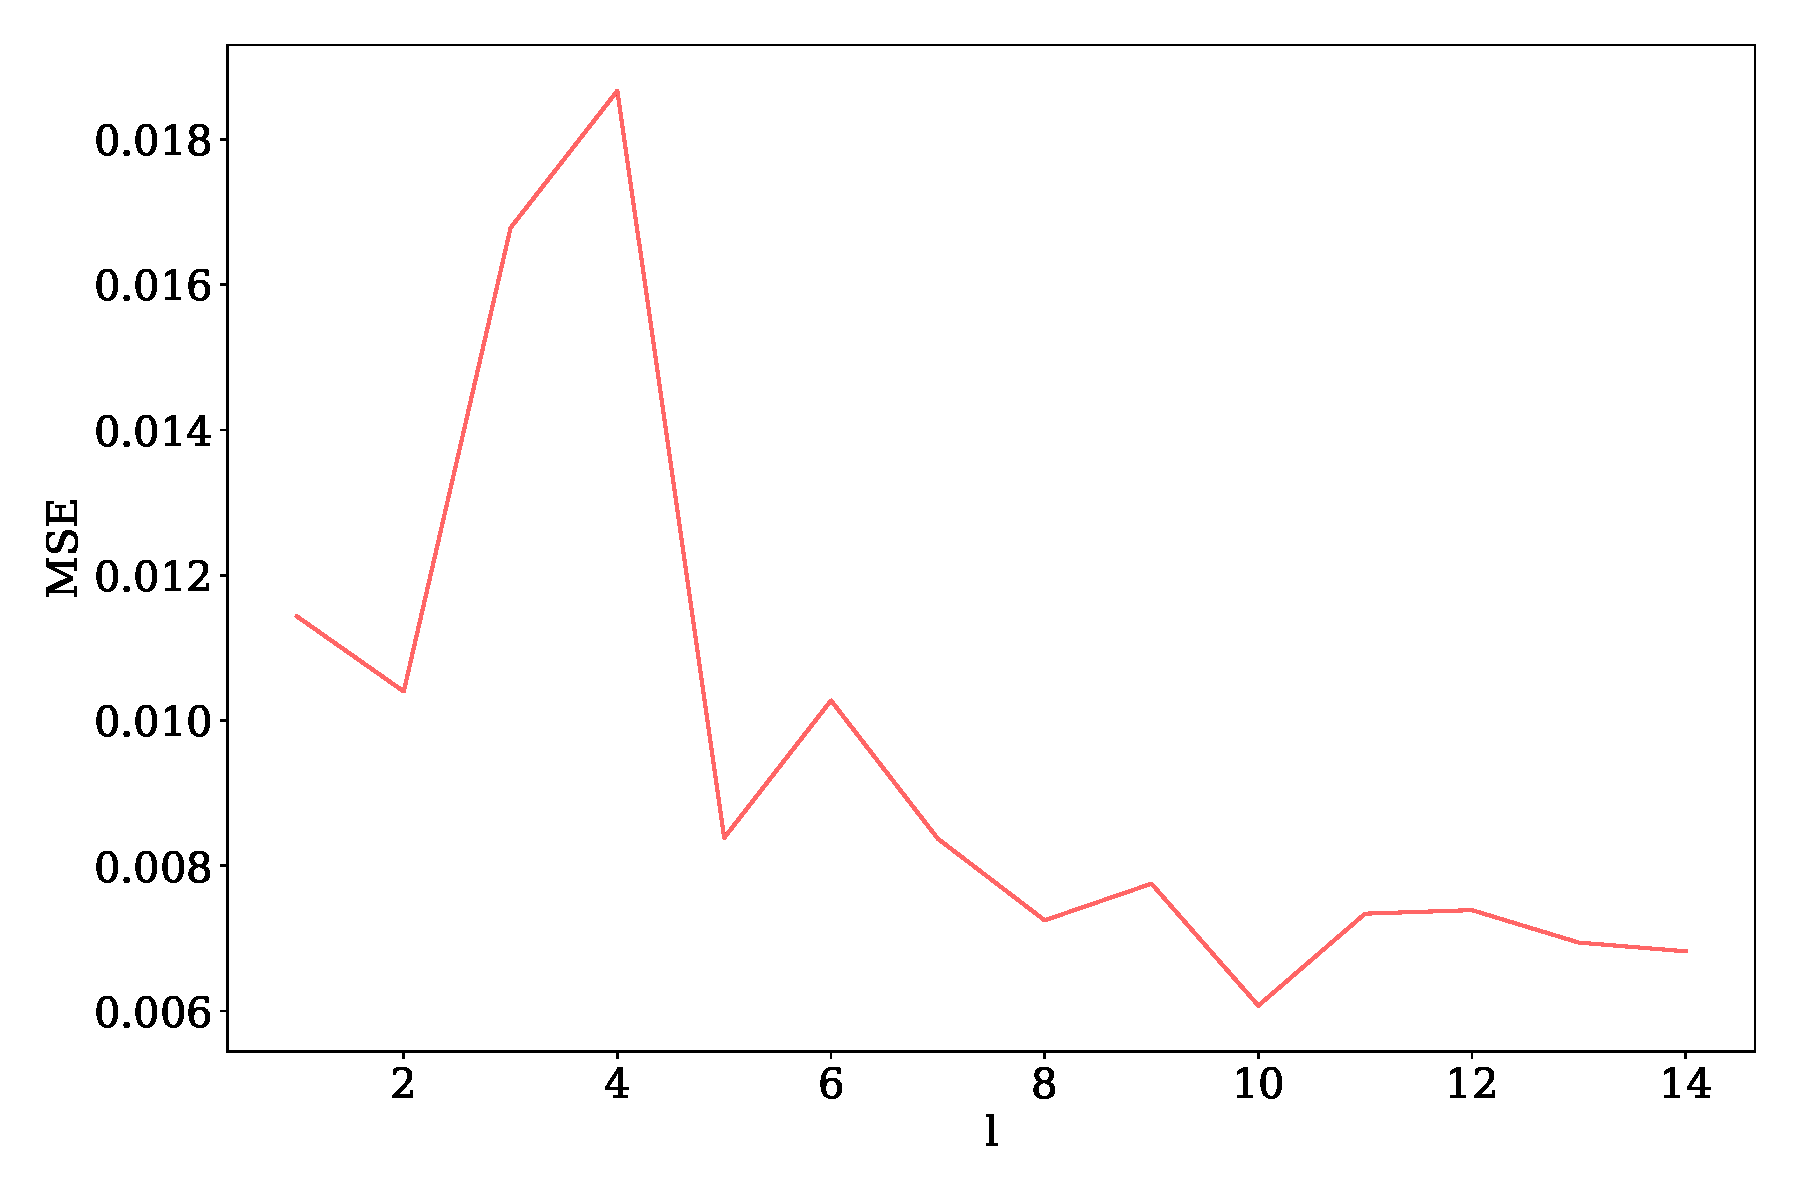
\includegraphics[width=0.5\textwidth]{barrido_en_l.pdf}
		\end{center}
		\caption{Valores de MSE en función del desfase usando una capa LSTM}
		\label{fig:barrido_en_l}
	\end{small}
\end{figure}
\end{document}